\section{Dise\~no de la metodolog\'ia}\label{dis}
Esta secci\'on se presenta todos los dise\~nos y c\'alculos matem\'aticos y estad\'isticos encontrados en los resultados. 
\subsection{Asignaci\'on de valores de etiquetas y rangos de identificaci\'on}\label{dis:asig}
Estos valores permiten identificar el paso de cada movimiento a partir de las siguientes variables:
\begin{itemize}
\item \textbf{Offset:} Valor de distribuci\'on de etiquetas de cada paso del movimiento, por partes iguales.
\begin{formula}[H]
	\centering
	\caption{Offset de etiquetas}
	\label{frm:offsetEt}
	\begin{equation}
offset = \frac{1}{pasos-1}
	\end{equation}
	\textbf{Fuente:} Propuesto por el autor de tesis
\end{formula}
\item \textbf{Vector de etiquetas:} A cada paso se le distribuye un valor \'unico, cuyo valor se calcula a partir del offset de la etiqueta anterior.
\begin{formula}[H]
	\centering
	\caption{Asignaci\'on de etiquetas}
	\label{frm:vecEtiq}
	\begin{equation}
\begin{matrix}
etiquetas=[0, etiqueta(1), ..., etiqueta(paso), ..., 1],\; donde
\\
\\
etiqueta(paso) =
\left\{\begin{matrix}
0 & Si\; es\; el\; primer \; paso
\\
etiqueta(paso-1)+offset & Si\; es\; un\; paso\; intermedio
\\ 
1 & Si\; es\; el\; \acute{u}ltimo\; paso
\end{matrix}\right.
\end{matrix}
	\end{equation}
	\textbf{Fuente:} Propuesto por el autor de tesis
\end{formula} 

\item \textbf{Valor de identificaci\'on:} N\'umero que representa la distribuci\'on de reconocimiento  de pasos por partes iguales:
\begin{formula}[H]
	\centering
	\caption{Valor de identificaci\'on de pasos}
	\label{frm:idenStep}
	\begin{equation}
valor \: de \: identificaci\acute{o}n = \frac{1}{pasos}
	\end{equation}
	\textbf{Fuente:} Propuesto por el autor de tesis
\end{formula} 

\item \textbf{Rango de identificaci\'on:} Rango m\'aximo num\'erico para identificar un paso.
\begin{formula}[H]
	\centering
	\caption{Rango m\'aximo de identificaci\'on de un paso}
	\label{frm:idenStep}
	\begin{equation}
\begin{matrix}
rango = [[inferior,superior]] \\
\\
rango(paso)=\left\{\begin{matrix}
inferior(paso)= \left\{\begin{matrix}
0 & paso\: inicial\\ 
superior(paso-1) & paso\: no\: inicial
\end{matrix}\right.\\ 
\\
superior(paso)= \left\{\begin{matrix}
inferior(paso)+identificaci\acute{o}n & paso\, no\, final\\ 
1 & paso\: final

\end{matrix}\right.\\ 
\end{matrix}\right.
\end{matrix}
	\end{equation}
	\textbf{Fuente:} Propuesto por el autor de tesis
\end{formula} 
\end{itemize}
\subsection{C\'alculo indirecto de la altura del usuario} \label{dis:height}
Para el presente proyecto se midi\'o la altura del usuario, a partir de la diferencia entre la altura de la cabeza y la altura promedio de los pies.
	\begin{formula}[H]
	\centering
	\caption{Altura del usuario}
	\label{frm:alturaUser}
	\begin{equation}
y_{usuario}=y_{cabeza}-\frac{y_{pie \: derecho}+y_{pie \: izquierdo}}{2}
	\end{equation}
			\textbf{Fuente:} Planteado por el autor de tesis
\end{formula} 
\subsection{C\'alculo de distancia de profundidad m\'inima y m\'axima} \label{dis:deep}
Para los siguientes c\'alculos se utilizaron la hoja de observaciones de profundidad (Ver anexo, tabla  \ref{tab:obsDepth}), aplicando las siguientes funciones de microsoft excel (versi\'on ingl\'es):
\begin{itemize}
       \item \textbf{Average}: Funci\'on para determinar la altura promedio.
\begin{formula}[H]
	\centering
	\caption{C\'alculo de altura promedio}
	\label{frm:avgHeight}
	\begin{equation}
	Altura \: promedio =AVERAGE([Altura])
	\end{equation}
		\textbf{Fuente:} Elaborado por el autor, a partir de funci\'on de excel
\end{formula}
       \item \textbf{Stdev}: Funci\'on para determinar la desviaci\'on est\'andar de la altura.
\begin{formula}[H]
	\centering
	\caption{C\'alculo de desviaci\'on est\'andar de la altura}
	\label{frm:stdevHeight}
	\begin{equation}
	desviaci\acute{o}n \:  de \: altura =STDEV([Altura])
	\end{equation}
		\textbf{Fuente:} Elaborado por el autor, a partir de funci\'on de excel
\end{formula}
       \item \textbf{Max}: Funci\'on para determinar la profundidad m\'axima entre el Kinect y el atleta.
       \begin{formula}[H]
	\centering
	\caption{C\'alculo de la profundidad m\'axima}
	\label{frm:maxDepth}
	\begin{equation}
	Profundidad \: Max =MAX([Profundidad])
	\end{equation}
		\textbf{Fuente:} Elaborado por el autor, a partir de funci\'on de excel
\end{formula}
       \item \textbf{Min}: Funci\'on para determinar la profundidad m\'inima entre el Kinect y el atleta.
              \begin{formula}[H]
	\centering
	\caption{C\'alculo de la profundidad m\'inima}
	\label{frm:minDepth}
	\begin{equation}
	Profundidad \:  Min =MIN([Profundidad])
	\end{equation}
		\textbf{Fuente:} Elaborado por el autor, a partir de funci\'on de excel.
\end{formula}
\end{itemize}
\subsection{Eventos del Kinect} \label{dis:even}
De acuerdo a la hoja de observaciones de extracci\'on de datos de v\'ideos (Ver tabla \ref{tab:obsVideoData}), se recupera la siguiente informaci\'on:
\begin{itemize}
\item \textbf{Eventos}: Conjunto de datos del seguimiento del esqueleto, durante un intervalo de tiempo.
\begin{formula}[H]
	\centering
	\caption{Matriz de eventos del Kinect}
	\label{frm:event}
	\begin{equation}
\begin{matrix}
Esqueleto & [SkeletonId, Joint, status, x, y, z] \\ 
Evento & [EventoIndex, TotalTime, esqueleto]  \\
\\ 
Eventos & 
\left.\begin{matrix}
Tiempo \: inicial\\ 
\\ 
\\
Tiempo \: final
\end{matrix}\right\}
\begin{matrix}
\left.\begin{matrix}
Evento \: inicial 
\end{matrix}\right\}\\ 
\left.\begin{matrix}
.. \\ 
Eventos \: no \: iniciales \\ 
 ..
\end{matrix}\right\}
\end{matrix}
\begin{bmatrix}
Evento_{0}\\ 
Evento_{1}\\ 
Evento_{2}\\ 
Evento_{x}
\end{bmatrix}
\end{matrix}
	\end{equation}
		\textbf{Fuente:} Propuesto por el autor de tesis.
\end{formula}
\item \textbf{Tiempo relativo}: Describe el tiempo de la repetici\'on, cuyo valor significa la diferencia entre el tiempo total de un evento no inicial y el tiempo total del primer evento.
              \begin{formula}[H]
	\centering
	\caption{C\'alculo del tiempo de la repetici\'on}
	\label{frm:relativeTime}
	\begin{equation}
	relative \: time = TotalTime_{Evento\: x}-TotalTime_{Evento\: inicial}
	\end{equation}
		\textbf{Fuente:} Propuesto por el autor de tesis.
\end{formula}
\item \textbf{Distancia euclidiana}: Describe el desplazamiento de una articulaci\'on, bas\'andose en la posici\'on del primer evento inicial y la posici\'on de un evento no inicial:
\begin{formula}[H]
	\centering
	\caption{Desplazamiento de una articulaci\'on}
	\label{frm:desplazaUser}
	\begin{equation}
|r|=\sqrt{(x_{joint}-x_{o})^{2}+(y_{joint}-y_{o})^{2}+(z_{joint}-z_{o})^{2}}
	\end{equation}
	\textbf{Fuente:} Distancia euclidiana \cite[p.~423]{ayres2001calculo}
\end{formula}  
\end{itemize}
As\'i mismo, con la herramienta de excel se realiz\'o un an\'alisis de regresi\'on  de los movimientos de animaci\'on y tenis de mesa, tomando en cuenta  la distancia recorrida de la mu\~neca -i.e. Variable independiente- y su respectivo tiempo -i.e. Variable dependiente-, a partir de una muestra de 10 a 15 repeticiones, con la finalidad de mostrar la uniformidad de los tiempos de capturas, la dispersi\'on de los datos de la muestra (diferentes desplazamientos) y calcular el tiempo de la repetici\'on m\'as larga (identifica el peor de los casos).
\subsection{Captura de datos durante una rutina (normalizaci\'on de datos)}\label{dis:recognitionMove}
Durante la rutina, los datos del seguimiento del esqueleto son recuperados a partir del kit de desarrollo de software del Kinect, dichos datos son almacenados en la siguiente estructura:
\begin{itemize}
\item \textbf{I:} Valor num\'erico \'unico que identifica una articulaci\'on.
\item \textbf{X:} Posici\'on horizontal de la articulaci\'on, dibujado en una imagen de dos dimensiones.
\item \textbf{Y:} Posici\'on vertical de la articulaci\'on, dibujado en una imagen de dos dimensiones.
\item \textbf{Fm:} Factor del movimiento proporcionado por la base de datos de gesturas.
\item \textbf{P:} Valor num\'erico que identifica el paso que est\'a realizando un atleta.
\item \textbf{Tiempo:} Tiempo de captura de datos.
\item \textbf{Joint:} Vector que almacena la posici\'on de una articulaci\'on en una figura de dos dimensiones.
\item \textbf{Esqueleto:} Vector que almacena todos los vectores de articulaciones del esqueleto humano.
\item \textbf{Step:} Vector que almacena informaci\'on del seguimiento del esqueleto, factor del movimiento y el tiempo de un paso.
\item \textbf{Repetici\'on:} Vector que almacena la informaci\'on de cada de paso de un movimiento.
\item \textbf{Serie:} Vector que almacena las repeticiones del movimiento durante una serie.
\item \textbf{Series:} Vector que almacena la informaci\'on de cada serie de la rutina.
\end{itemize}
\begin{formula}[H]
	\centering
	\caption{Matriz de datos capturados durante una rutina}
	\label{frm:MatrizDatosRepeticion}
	\begin{equation}
\begin{matrix}
i & enumerador\: de\: la\: articulaci\acute{o}n \\ 
x & distancia\, horizontal \: (p\acute{i}xeles) \\ 
y & distancia\, vertical\: (p\acute{i}xeles) \\ 
joint_{i}& [i,x,y] \\ 
 & \\ 
esqueleto & \begin{bmatrix}
joint_{0} \\ 
... \\ 
joint_{i}\\ 
... \\ 
joint_{24}
\end{bmatrix}  \\ 
 & \\ 
fm & factor \, del \, movimiento \\ 
p  & paso \, del \,movimiento \\ 
t  & tiempo \, total \\ 
step_{p}  & [fm,p,esqueleto, tiempo] \\
 & \\ 
Repeticion & [step_{0}, ...,  step_{col}, ..., step_{last}] \\
serie & [repeticion] \\
series & [serie]
\end{matrix}
	\end{equation}
	\textbf{Fuente:} Propuesto por el autor de tesis
\end{formula}
\subsection{Validaci\'on del modelo de reconocimiento de movimiento}\label{dis:validate}
El presente proyecto se utiliz\'o dos m\'etodos de validaciones cruzadas \cite{perez2015analisis}:
\begin{itemize}
\item \textbf{Hold out:} Las muestras de datos se separan en dos conjunto, uno para construir y entrenar el modelo -i.e. Build- y otro para realizar pruebas que dan validez a los m\'argenes  de errores del modelo.
\item \textbf{K-fold:} Las muestras se dividen en K subconjuntos, y en cada subconjunto se aplica el m\'etodo hold out.
\end{itemize}  
\begin{table}[H]
\begin{center}
\caption{Validaci\'on cruzada, 3-fold de tenis de mesa}
\label{tab:KfoldTenis}
\begin{tabular}{|l|l|l|}
\hline
\multicolumn{3}{|c|}{\textbf{Muestra de v\'ideos}} \\ \hline
\multicolumn{3}{|c|}{1, 2, 3, 4, 5, 6} \\ \hline
\textbf{Modelo} & \textbf{Builds} & \textbf{Test} \\ \hline
1 & 1, 2, 3, 4, 5 & 6 \\ \hline
2 & 1, 2, 4, 5, 6 & 3 \\ \hline
3 & 2, 3, 4, 5, 6 & 1 \\ \hline
\multicolumn{3}{l}{\textbf{Fuente:} Propia}
\end{tabular}
\end{center}
\end{table}
\begin{table}[H]
\begin{center}
\caption{Validaci\'on cruzada, 3-fold de animaci\'on}
\label{tab:KfoldAnimacion}
\begin{tabular}{|l|l|l|}
\hline
\multicolumn{3}{|c|}{\textbf{Muestra de v\'ideos}} \\ \hline
\multicolumn{3}{|c|}{1, 2, 3, 4, 5, 6, 7} \\ \hline
\textbf{Modelo} & \textbf{Builds} & \textbf{Test} \\ \hline
1 & 1, 2, 3, 4, 5, 6 & 1 \\ \hline
2 & 1, 2, 3, 5, 6, 7 & 4 \\ \hline
3 & 1, 2, 3, 4, 5, 6 & 7 \\ \hline
\multicolumn{3}{l}{\textbf{Fuente:} Propia}
\end{tabular}
\end{center}
\end{table}
\begin{table}[H]
\begin{center}
\caption{Validaci\'on cruzada, 3-fold de taekwondo}
\label{tab:KfoldTaekwondo}
\begin{tabular}{|l|l|l|}
\hline
\multicolumn{3}{|c|}{\textbf{Muestra de videos}} \\ \hline
\multicolumn{3}{|c|}{1, 2, 3, 4, 5, 6, 7, 8, 9, 10, 11, 12, 13, 14, 15, 16} \\ \hline
\textbf{Modelo} & \textbf{Builds} & \textbf{Test} \\ \hline
1 & 1, 2, 3, 4, 5, 6, 7, 8, 9, 11, 12, 13, 14, 15, 16 & 10 \\ \hline
2 & 1, 2, 3, 4, 5, 6, 7, 8, 9, 10, 12, 13, 14, 15, 16 & 11 \\ \hline
3 & 1, 2, 3, 4, 5, 6, 7, 8, 9, 10, 11, 13, 14, 15, 16 & 12 \\ \hline
\multicolumn{3}{l}{\textbf{Fuente:} Propia}
\end{tabular}
\end{center}
\end{table}
Posteriormente en la etapa de pruebas, se realiz\'o  por cada modelo una hoja de observaciones de valores reales y pronosticados (ver anexo, tabla \ref{tab:obsErrores}), de modo de encontrar los siguientes errores de pron\'osticos \cite{erroresPronostico}:
\begin{itemize}
\item \textbf{Error medio pronosticado (\acrshort{EMP}):} Promedio de diferencia entre el valor real y pronosticado, la cual puede tener tres interpretaciones distintas:
	\begin{itemize}
	\item \textbf{Valor positivo:} En promedio, los valores pronosticado est\'an por debajo de los valores reales.
	\item \textbf{Valor negativo:} En promedio, los valores pronosticado est\'an por arriba de los valores reales.
	\item \textbf{Valor cero:} Los valores pronosticados pueden estar por debajo o por arriba de los valores reales.
	\end{itemize}
\begin{formula}[H]
	\centering
	\caption{C\'alculo del error medio pronosticado}
	\label{frm:empMath}
	\begin{equation}
EMP=\frac{\sum_{0}^{n}(Real_{x}-Pronostic_{x}\cdot10^{-6})}{n}
	\end{equation}
	\textbf{Fuente:} Formula adaptada al proyecto, a partir de la f\'ormula del error medio pronosticado \cite{videoErrores}
\end{formula}  
\item \textbf{Desviaci\'on media absoluta (\acrshort{DMA}):} Promedio de diferencia absoluta entre el valor real y pronosticado, que muestra la dispersi\'on con respecto al valor real.
 \begin{formula}[H]
	\centering
	\caption{C\'alculo de la desviaci\'on media absoluta}
	\label{frm:MADMath}
	\begin{equation}
DMA=\frac{\sum_{0}^{n}( \left |  Real_{x}-Pronostic_{x}\cdot10^{-6} \right |)}{n}
	\end{equation}
	\textbf{Fuente:} Formula adaptada al proyecto, a partir de la f\'ormula de la desviaci\'on media absoluta \cite{videoErrores}
\end{formula}  
\item \textbf{Ra\'iz del error cuadr\'atico medio (RECM):} Es la desviaci\'on est\'andar de los errores de predicci\'on, la cual indica qu\'e tan disperso se encuentra los errores con respecto al error medio pronosticado.
 \begin{formula}[H]
	\centering
	\caption{C\'alculo de la ra\'iz del error cuadr\'atico medio}
	\label{frm:RECMMath}
	\begin{equation}
RECM=\sqrt{\frac{\sum_{0}^{n}((Real-Pronostic\cdot10^{-6})-EMP)^{2}}{n}}
	\end{equation}
	\textbf{Fuente:} Formula adaptada al proyecto, a partir de la f\'ormula de la ra\'iz del error cuadr\'atico medio \cite{GEORCMETUT}
\end{formula}  
\end{itemize}
Luego de encontrar los errores, se debe seleccionar el modelo que tenga la menor \acrshort{RECM}, y posteriormente encontrar los errores de la muestra total:
 \begin{formula}[H]
	\centering
	\caption{EMP de la muestra total}
	\label{frm:EmpAll}
	\begin{equation}
EMP_{muestra\, total}=AVERAGE([EMP_{modelo}])
	\end{equation}
	\textbf{Fuente:} Propuesto por el autor de tesis, con base a las f\'ormulas de excel (versi\'on en ingl\'es)
\end{formula}  
 \begin{formula}[H]
	\centering
	\caption{MAD de la muestra total}
	\label{frm:MadAll}
	\begin{equation}
MAD_{muestra\, total}=AVERAGE([MAD_{modelo}])
	\end{equation}
	\textbf{Fuente:} Propuesto por el autor de tesis, con base a las f\'ormulas de excel (versi\'on en ingl\'es)
\end{formula}  
	 \begin{formula}[H]
	\centering
	\caption{RECM de la muestra total}
	\label{frm:RecmAll}
	\begin{equation}
RECM_{muestra\, total}=AVERAGE([RECM_{modelo}])
	\end{equation}
	\textbf{Fuente:} Propuesto por el autor de tesis, con base a las f\'ormulas de excel (versi\'on en ingl\'es)
\end{formula} 
Los errores de la muestra total ayudan aceptar o rechazar el modelo; si la \acrshort{RECM} promedio  es menor a un medio del valor de identificaci\'on se aprueba (se divide entre dos, debido que las etiquetas de los pasos intermedio se encuentra a la mitad de cada rango de identificaci\'on respectiva). En caso que sea mayor o igual, se rechaza, debido que los intervalos de confianza colisiona con otros intervalos de confianza (Intervalos que se utiliza para la detecci\'on de un paso):
\begin{figure}[H]
	\caption{Criterios de aceptaci\'on de un modelo de detecci\'on de los pasos requeridos de un movimiento}
	\label{fig:AproveOrDennie}
	\centering
	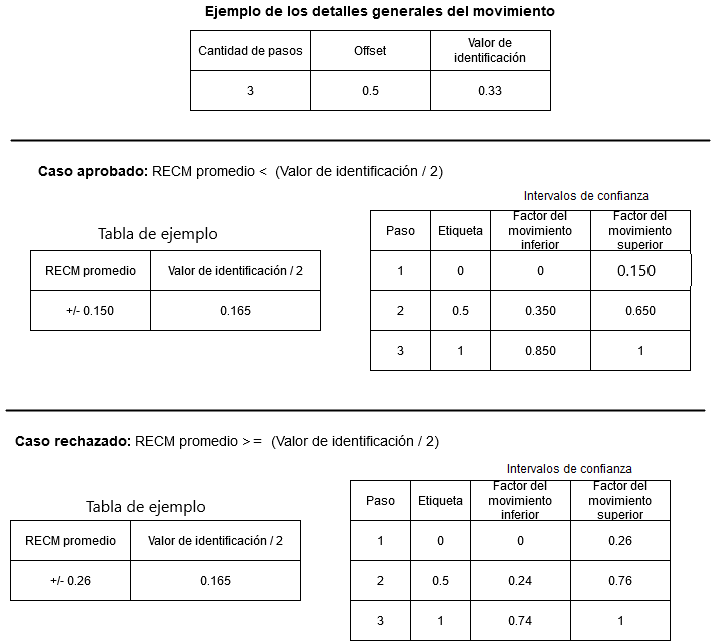
\includegraphics[width=430px,height=360px]{graphics/CriterioAceptacion.png} \\
	\textbf{Fuente:} Propia
\end{figure}
En la figura \ref{fig:AproveOrDennie}, se separa en tres partes:
\begin{itemize}
\item \textbf{Detalles generales del movimiento:} Muestra las variables num\'ericas de un movimiento.
\item \textbf{Caso aprobado:} Al construir los intervalos de confianza, se observa que no colisiona entre s\'i.
\item \textbf{Caso rechazado:} Al construir los intervalos de confianza, se observa que los intervalos del paso 1 colisiona con el paso 2 (debido que el intervalo de confianza inferior del paso 2 se encuentra dentro del intervalo de confianza del paso 1), y los intervalos del paso 2 colisiona con el paso 3 (debido que el intervalo de confianza inferior del paso 3 se encuentra dentro del intervalo de confianza del paso 2).
\end{itemize}
Adem\'as, por cada modelo aprobado se debe encontrar los intervalos de confianza  que permite detectar los pasos de un movimiento v\'alido:
\begin{formula}[H]
	\centering
	\caption{Intervalos de confianza de reconocimiento de un paso}
	\label{frm:rangoConfiabilidad}
	\begin{equation}
\begin{matrix}

intervalo\: de\: confianza = ic =[[inferior,superior]] \\
\\
ic(paso)=\left\{\begin{matrix}
inferior(paso)=\left\{\begin{matrix}
0 & si\, es\, el\, primer\, paso\\ \\ 
etiqueta(paso)- RECM_{muestra\, total} & si\: es\: paso\: intermedio \\ 
\\
1-RECM_{muestra\, total}& si\, es\, el\, \acute{u}ltimo\, paso
\end{matrix}\right. \\ 
\\ 
inferior(paso)=\left\{\begin{matrix}
RECM_{muestra\, total}& si\, es\, el\, primer\, paso \\
\\
etiqueta(paso)+RECM_{muestra\, total} & si\: es\: paso\: intermedio \\ \\ 
1 & si\: es\: el\: \acute{u}ltimo\: paso
\end{matrix}\right.
\end{matrix}\right.
\end{matrix}
	\end{equation}
	\textbf{Fuente:} Propuesto por el autor de tesis
\end{formula} 
Por otro lado, se debe determinar el valor de recognition, n\'umero porcentual que determina el porcentaje de detecci\'on similar al fotograma de cada paso respectivo, es decir:
 \begin{itemize}
\item \textbf{Porcentaje mayor a cero:} Entre m\'as cercano al 100\%, el factor de movimiento es similar al valor de etiquetado (menor error).
\item \textbf{Porcentaje menor o igual a cero:} Son modelos rechazado, debido que el error es grande y adem\'as no detecta los pasos de un movimiento (por colisiones de los intervalos de confianza).
\end{itemize}
\begin{formula}[H]
	\centering
	\caption{Valor de recognition}
	\label{frm:Recognitiona}
	\begin{equation}
recognition=1-no\,v\acute{a}lidos=1-\frac{RECM_{muestra\, total}}{valor\: de\: identificaci\acute{o}n}  
	\end{equation}
	\textbf{Fuente:} Propuesto por el autor de tesis
\end{formula}
\subsection{Algoritmo clasificador de un movimiento v\'alido}\label{dis:algoritmoDet}
Se presenta el algoritmo clasificador de repetici\'on de un movimiento v\'alido:
\begin{itemize}
\item Entradas:
\begin{itemize}
\item \textbf{Paso siguiente:} Variable que lleva el control del orden de todos los pasos detectados.
\item \textbf{Factor del movimiento:} Variable que indica la transici\'on del movimiento a partir del algoritmo Random Forest Regression.
\item \textbf{Paso detectado:} Variable que indica el paso actual del factor del movimiento.
\item \textbf{Paso no detectado:} Variable que no tiene un valor al inicio, la cual se asigna un valor en el caso que sea una repetici\'on inv\'alida (indica el paso del fallo del movimiento).
\end{itemize}
\item Procesos:
\begin{enumerate}[1.]
\item Asignar el paso siguiente como paso inicial (paso No.1), debido que marca el inicio de la repetici\'on. %1
\item Capturar un nuevo fotograma del Kinect, y obtiene el factor del movimiento del respectivo fotograma, a partir del algoritmo Random Forest Regression y la herramienta, Visual Gesture Builder. %2
\item Verificar si el factor del movimiento se encuentra en alg\'un intervalo de confianza para obtener el paso detectado, en caso que no se encuentre, no devolver\'a ning\'un valor.  %3
\item Verificar si el paso detectado tiene un valor y que no sea un valor anterior (valor anterior del paso siguiente), en caso que no sea, se debe esperar a capturar un nuevo fotograma (Volver al proceso No.2). %4
\item Verificar si el paso detectado es igual al paso siguiente, en caso que sea diferente se detect\'o una repetici\'on inv\'alida (saltar al proceso No. 9). %5
\item Verificar si el paso detectado es el \'ultimo paso, en caso contrario (saltar al proceso No. 8) %6
\item Finalizar algoritmo con repetici\'on v\'alida. %7 
\item Incrementar el paso siguiente y volver a obtener un nuevo fotograma del Kinect (saltar al proceso No. 2). %8
\item Asignar el paso no detectado como paso siguiente.
\item Finalizar el algoritmo con repetici\'on inv\'alida.
\end{enumerate}
\item Salidas:
\begin{itemize}
\item \textbf{Repetici\'on v\'alida:} El usuario pas\'o por todos los pasos de un movimiento v\'alido de forma ordenada.
\item \textbf{Repetici\'on inv\'alida y su paso no detectado:} El usuario se salt\'o el paso no detectado, lo cual genera un movimiento inv\'alido.
\end{itemize}
\end{itemize}
\begin{figure}[H]
	\caption{Algoritmo clasificador de repetici\'on de un movimiento v\'alido }
	\label{fig:capturaDatos}
	\centering
	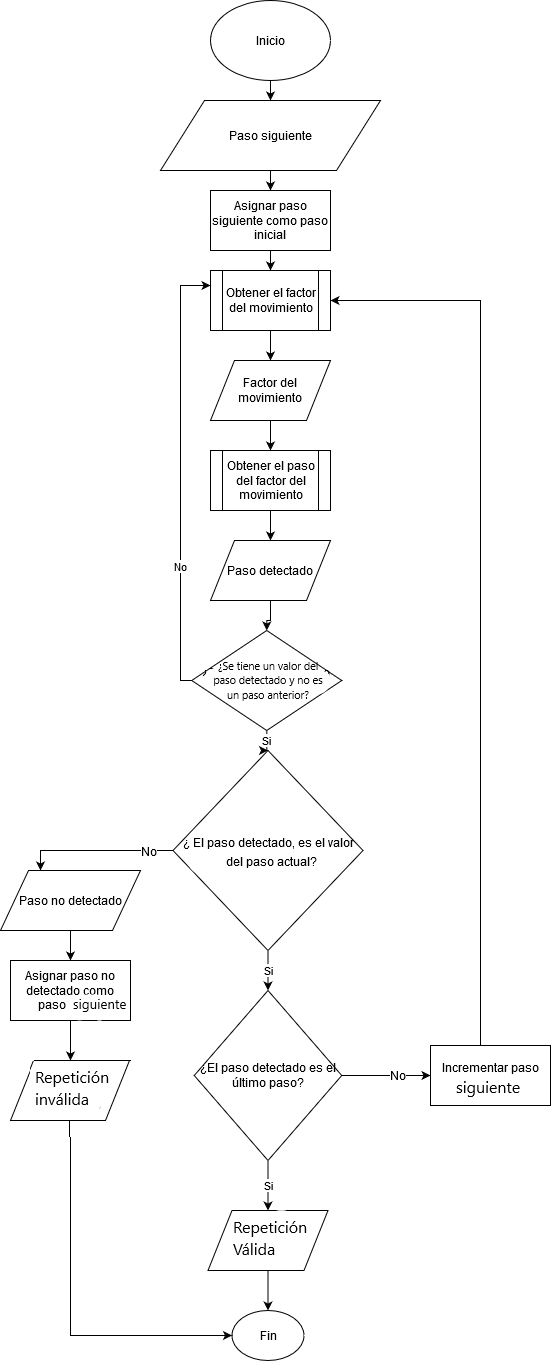
\includegraphics[width=430px,height=630px]{graphics/flujoGramaRepiticion.png} \\
	\textbf{Fuente:} Propia.
\end{figure}
Este algoritmo es aplicado para analizar los v\'ideos de testeos, debido que se etiquetaron  repeticiones de movimientos v\'alidos.  Sin embargo, al comparar los factores del movimiento de los fotogramas (de los v\'ideos de testeos), pueden ocurrir que no reconozca un paso, por lo tanto la repetici\'on del movimiento v\'alido se convierte en inv\'alido:
 \begin{figure}[H]
	\caption{Clasificaci\'on de repeticiones de movimiento v\'alido o inv\'alido  en un v\'ideo de testeo}
	\label{fig:detValido}
	\centering
	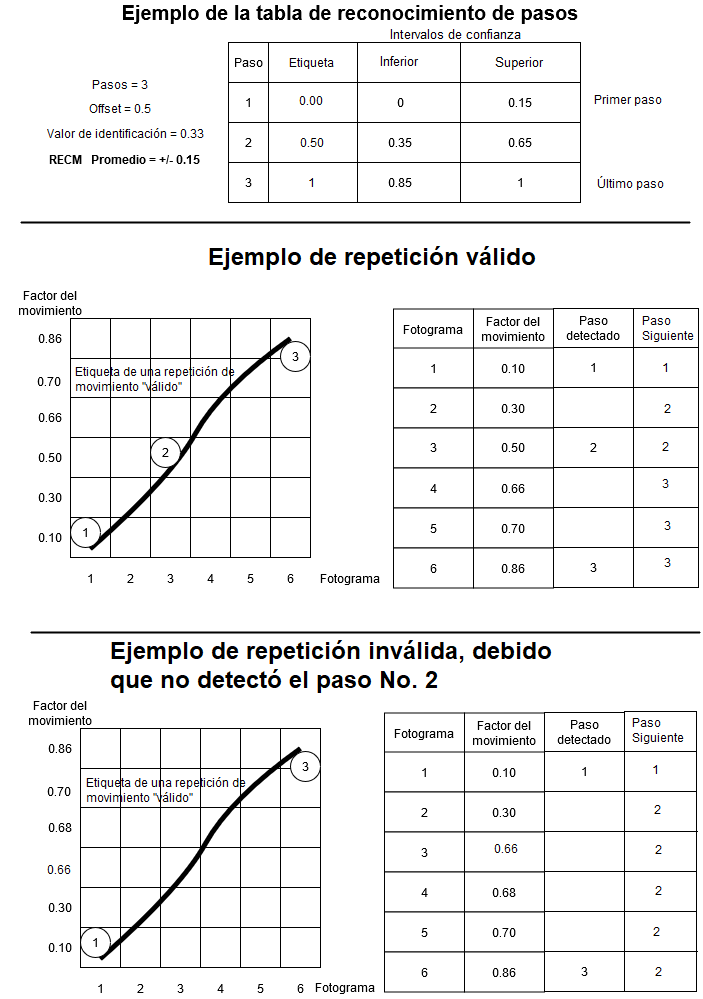
\includegraphics[width=430px,height=450px]{graphics/reconocimientoDePasos.png} \\
	\textbf{Fuente:} Propia.
\end{figure}
En la figura \ref{fig:detValido}, se divide en tres partes:
\begin{itemize}
\item \textbf{Intervalos de confianza:} Tabla que permite reconocer los pasos del movimiento, si el factor del movimiento se encuentra dentro del intervalo de confianza.
\item \textbf{Repetici\'on v\'alida:} Es v\'alido,  ya que detecta todos los pasos de manera ordenada  durante los fotogramas: Uno, tres y seis (Observe que los factores del movimiento se encuentran dentro del alg\'un intervalo de confianza). 
\item \textbf{Repetici\'on inv\'alida:} Es inv\'alido, debido que para el fotograma 6, se esperaba detectar el paso 2 (paso siguiente), pero se detect\'o el paso 3, por lo tanto el algoritmo determina que es una repetici\'on inv\'alida.
\end{itemize}
Este procedimiento permite completar la tabla de observaciones de clasificaci\'on de cada v\'ideo de testeo (Tabla \ref{tab:DetectarPasoCorrecto}), en donde por cada repetici\'on etiquetada se verifica todos los pasos, por medio de tres valores:
\begin{itemize}
\item \textbf{Verdadero:} Si se detect\'o el paso correspondiente (de manera ordenada).
\item \textbf{Falso:} Repetici\'on invalida debido que no se detect\'o el paso correspondiente. 
\item \textbf{Sin valor:} El algoritmo no determin\'o ning\'un valor, debido que finaliz\'o al momento  que detect\'o una repetici\'on inv\'alida.
\end{itemize}
Por otra parte, se puede determinar el porcentaje de v\'alido e inv\'alidos del modelo de clasificador de repeticiones, adem\'as de determinar el porcentaje de cada paso no detectado:
\begin{formula}[H]
	\centering
	\caption{Porcentajes del modelo de clasificador}
	\label{frm:porcentajeClasificador}
	\begin{equation}
\begin{matrix}
repeticiones\: v\acute{a}lidas = contarSi(\acute{u}ltimo\: paso\: es\: verdadero) \\ 
 \\ 
repeticiones\: inv\acute{a}lidas = repeticiones\; totales\: del\: video - repeticiones\: v\acute{a}lidas\\ 
 \\ 
\%_{v\acute{a}lidos}=\frac{repeticiones\: v\acute{a}lidas}{repeticiones\; totales\: del\: video}\\ 
\\
\%_{inv\acute{a}lidos}=\frac{repeticiones\: inv\acute{a}lidas}{repeticiones\; totales\: del\: video}\\ 
\\ 
\%_{paso\; no\; detectado}=\frac{contarSi(paso\: es\: falso)}{repeticiones\: inv\acute{a}lidas}\\ 
\end{matrix}
	\end{equation}
	\textbf{Fuente:} Propuesto por el autor de tesis
\end{formula}
Es importante saber si el modelo de clasificaci\'on  de un movimiento v\'alido se aprueba, por lo tanto se debe calcular los porcentajes de referencias v\'alido e inv\'alido, que se determinan a partir del peor de los casos (detecta una repetici\'on v\'alida y las permutaciones de las  repeticiones inv\'alidas): 
 \begin{figure}[H]
	\caption{Porcentajes de referencias v\'alidos e inv\'alidos }
	\label{fig:porcValido}
	\centering
	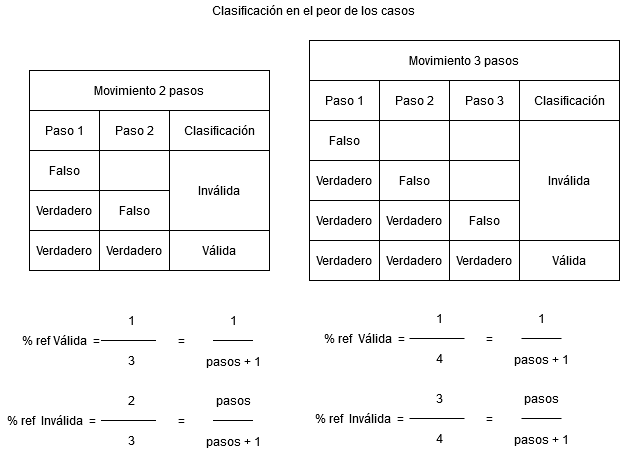
\includegraphics[width=430px,height=300px]{graphics/porceRef.png} \\
	\textbf{Fuente:} Propia.
\end{figure}
A partir de los porcentajes de referencias de clasificaci\'on, se pueden presentar dos casos:
\begin{itemize}
\item \textbf{Clasificaci\'on Aceptable:} Si el porcentaje de detecci\'on v\'alida es mayor al porcentaje de referencia v\'alida (Por consiguiente el porcentaje de detecci\'on inv\'alida es menor al porcentaje de referencia inv\'alida).
\item \textbf{Clasificaci\'on no aceptable:} Si el porcentaje de detecci\'on v\'alida es menor o igual al porcentaje de referencia v\'alida (Por consiguiente el porcentaje de detecci\'on inv\'alida es mayor o igual al porcentaje de referencia inv\'alida). 
\end{itemize}
\subsection{Dise\~no de los resultados de una rutina tabata} \label{dis:results}
En esta secci\'on se determina los resultados de la rutina de tabata, dichos resultados son encontrados a partir del seguimiento del esqueleto, la cual proporciona informaci\'on de las variables de los detalles del paso y repetici\'on (Ver f\'ormula \ref{frm:MatrizDatosRepeticion}), con el fin objetivo de encontrar la siguiente informaci\'on:
\begin{itemize}
\item \textbf{Volumen de repeticiones:} Sumatoria de las cantidades totales de repeticiones de una serie.  
\begin{code}[H]
	\caption{Pseudoc\'odigo para obtener las repeticiones totales de una rutina}
	\label{code:getRepetitions}
	\begin{lstlisting}
Entradas:
	Series de repeticiones del movimiento
	Contador de Repeticiones

Procesos:
	Recorrer cada serie de repeticiones del movimiento:
		Contar las repeticiones de la serie
		Sumar al contador de repeticiones

Salida:
	Contador de repeticiones
	\end{lstlisting}
	\textbf{Fuente:} Propia.
\end{code}

\item \textbf{Duraci\'on:} Tiempo total que se emplea en una rutina, tomando en cuenta todas las series de trabajos y descansos.
\begin{formula}[H]
	\centering
	\caption{C\'alculo de la duraci\'on de tiempo de una rutina}
	\label{eq:DurationTime}
	\begin{equation}
	Duration = \sum_{i=0}^{series}restTime +\sum_{i=0}^{series}workTime = series(restTime+workTime)
	\end{equation}
		\textbf{Fuente:} Elaborado por el autor de tesis
\end{formula}
\item \textbf{Resistencia:} Construye la estructura de la gr\'afica de la resistencia de un atleta durante una rutina a partir del recorrido de todas la series, posteriormente en cada serie se recorre todas las repeticiones y luego en cada repetici\'on se almacena el tiempo acumulado de la rutina y la cantidad de repeticiones que lleva el atleta a ese momento.
\begin{code}[H]
	\caption{Pseudoc\'odigo para crear la gr\'afica de resistencia}
	\label{code:getEndurance}
	\begin{lstlisting}
Entradas:
	Series de repeticiones del movimiento
	Gráfico en donde almacena
		Subgráfico que está compuesto por
			Nombre de la serie
			Listado de puntos en donde cada punto
				Guarda el tiempo (eje x)
				Guarda el numero de repetición (eje y)
	
Proceso:
	Crear gráfico
	Recorrer cada serie de repeticiones del movimiento
		Crear subgráfico
		Obtener el número de serie
		Crear el listado de puntos
		Recorrer cada repetición de la serie
			Obtener el número de repeticiones acumuladas 
			Obtener el tiempo del paso final de la repetición
			Crear un punto
			Guardar punto en el listado de puntos
		Almacenar en el subgráfico el número de serie y listado de puntos
		Guardar subgráfico en el listado que tiene el gráfico

Salida:
	Gráfico de resistencia
	\end{lstlisting}
	\textbf{Fuente:} Propia.
\end{code} 

\item \textbf{Potencia:} Resultado que muestra la cantidad m\'axima de repeticiones en el menor tiempo posible, la cual se encuentra a partir del recorrido de las series, luego en cada serie se determina la cantidad de repeticiones totales y el tiempo acumulado de la \'ultima repetici\'on, encontrando: 
	\begin{itemize}
	\item Una mayor cantidad de repeticiones almacenada anteriormente
	\item La misma cantidad de repeticiones almacenada anteriormente, pero se verifica si el tiempo acumulado es menor.
	\end{itemize}
\begin{code}[H]
	\caption{Pseudoc\'odigo para obtener la potencia}
	\label{code:getEndurance}
	\begin{lstlisting}
Entradas:
	Series de repeticiones del movimiento
	Potencia en donde almacena
		Cantidad de repeticiones acumuladas de una serie
		Tiempo total de la última repetición de la serie
		
Procesos:
	Crear potencia
	Recorrer cada serie de repeticiones del movimiento
		Obtener la última repetición de la serie
			Obtener el número de repeticiones acumuladas
			Obtener el tiempo del paso final de la repetición
			¿El número de repeticiones acumuladas aumentó?
				Si
					Almacenar los datos en potencia
				Sino si, ¿El número de repeticiones permaneció igual?:
					¿El Tiempo total disminuyó?:
						Si
							Almacenar los datos en potencia
						
Salida:
	Potencia 
	\end{lstlisting}
	\textbf{Fuente:} Propia.
\end{code} 

\item \textbf{Velocidad}: Raz\'on de cambio separado por:
	\begin{itemize}
	\item \textbf{Repeticiones por serie:} Variable que se determina a partir del promedio total de repeticiones por serie.
		\item \textbf{Tiempo por repetici\'on:} Variable que se determina a partir del promedio de la diferencia entre el tiempo del paso final y tiempo del paso inicial -i.e. Tiempo de una repetici\'on- de cada repetici\'on realizada por el atleta.
	\end{itemize}
\end{itemize}


\begin{code}[H]
	\caption{Pseudoc\'odigo para obtener las velocidades de las rutinas}
	\label{code:getTimeOfRepetitions}
	\begin{lstlisting}
Entradas:
	Series de repeticiones del movimiento
	Velocidad en donde almacena
		Repeticiones por serie
		Tiempo por serie
		
Proceso:
	Crear velocidad
	Crear un listado de tiempos de repeticiones
	Crear un listado de repeticiones de series
	Recorrer cada serie de repeticiones del movimiento
		Obtener el total de repeticiones de la serie
		Agregar al listado de repeticiones de series
		Recorrer cada repetición de la serie
			Obtener el tiempo del paso inicial de la repetición
			Obtener el tiempo del paso final de la repetición
			Encontrar la diferencia de tiempos del paso final e inicial
			Almacenar en el listado de tiempos de repeticiones
	Encontrar el promedio de repeticiones de series
	Transformar a número entero el promedio de repeticiones de series
	Encontrar el promedio de tiempos de repeticiones
	Almacenar ambos promedios en velocidad
	
Salida:
	Velocidad
	\end{lstlisting}
	\textbf{Fuente:} Propia.
\end{code} 
\section{Criterios del proyecto}\label{criter}
En esta secci\'on se presenta todos los criterios que se siguieron para crear el modelo de reconocimientos de movimientos:
\subsection{Criterios de selecci\'on de movimiento}
\begin{itemize}
	\item El investigador y el entrenador de cada deporte  seleccionaron aquellos movimientos que se ejecutan dentro del \'area de visi\'on del sensor Kinect.
	\item El movimiento no debe ser complejo, es decir que cualquier persona pueda realizar dicho movimiento, sin importar su nivel deportivo.
	\item Debe ser un movimiento que se emplea constantemente en el deporte, para aprender nuevos movimientos complejos.
\end{itemize}
\subsection{Criterios de an\'alisis de movimiento}
\begin{itemize}
	\item Cada movimiento debe tener una articulaci\'on de an\'alisis.
	\item El conjunto de articulaciones que interact\'uan en el movimiento, se debe seleccionar con base a la separaci\'on del cuerpo humano, es decir, la parte inferior (Articulaciones abajo de la cadera central) o superior (Articulaciones arriba de la cadera central).
\end{itemize}
\subsection{Criterios de etiquetaci\'on de movimiento}
\begin{itemize}
	\item Cada repetici\'on del movimiento debe pasar por todos los pasos.
	\item El rango de etiquetaci\'on debe estar entre valores de 0 (paso inicial) y 1 (paso final).
	\item La curva de aprendizaje de cada repetici\'on, debe ser similar a la funci\'on sigmoide -i.e. gr\'afica con forma de ese (s)-.
	\item No se etiqueta los datos de ruidos durante una repetici\'on del movimiento -e.g. Interrupciones, errores en el seguimiento del esqueleto-.
\end{itemize}
\subsection{Criterios de error del modelo}
\begin{itemize}
	\item Se debe calcular la dispersi\'on entre los datos de la muestra y su media, a partir de la ra\'iz del error cuadr\'atico medio (RECM).
	\item Se debe calcular la dispersi\'on entre los datos reales y pronosticado a partir de la desviaci\'on media absoluta (DMA). 
	\item El error se encuentra en un rango de 0 a 1.
\end{itemize}
\subsection{Criterios de selecci\'on del modelo}
\begin{itemize}
	\item Se selecciona el submodelo que contenga la  menor RECM, en caso que exista RECM iguales, se escoge el modelo que tenga la menor DMA.
\end{itemize}
\subsection{Criterios de aceptaci\'on del modelo}
\begin{itemize}
	\item El modelo seleccionado debe considerar los errores de todas las muestras, a partir del promedio de errores de los submodelos comparados.
	\item Se aprueba el modelo, s\'i el valor promedio de la RECM es menor a un medio del valor de  identificaci\'on.
\end{itemize}